\documentclass[answers]{exam}
\usepackage{texPreamble}
\usepackage{relsize}
\usepackage{tabularx}
\extraheadheight{0.25in}
\extrafootheight{1.0in}
\extrawidth{1in}
% ----------------------------------------------------------------
\firstpagefootrule
\runningfootrule
\begin{document}
%\relscale{1.4}
\section{4.6: Linear Approximation and Differentials}
\begin{ex*}
  Find the equation of the line tangent to $f(x)=1+\sin(x)$ at $a=0$. State the line in the slope--intercept form.
\end{ex*}
\vspace*{\stretch{1}}
\begin{flushright}
  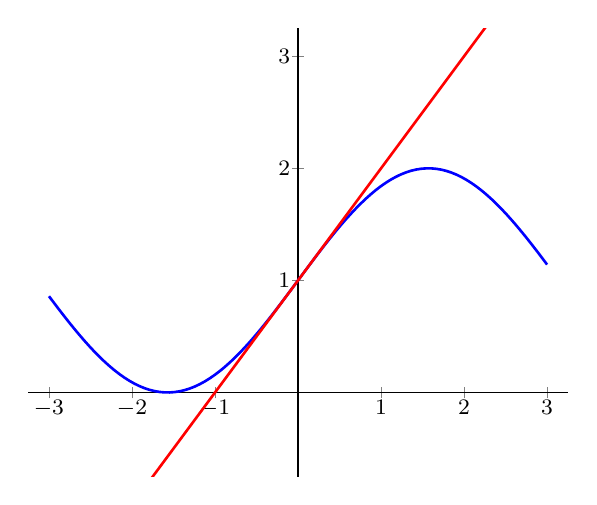
\begin{tikzpicture}
    \begin{axis}[
      grid style={line width=0.35pt, draw=gray!75},
      axis lines=center,
      axis line style={-},
      xmin=-3.25, xmax=3.25,
      ymin=-0.75, ymax=3.25,
      xtick={-6,-5,...,6},
      ytick={-6,-5,...,6},
      ticklabel style={font=\footnotesize,inner sep=0.5pt,fill=white,opacity=1.0, text opacity=1},
      every axis plot/.append style={line width=0.95pt, color=blue, samples=100}
      ]
      \addplot[-] expression[domain=-3:3]{1+sin(deg(x))};
      \addplot[-] expression[red]{x+1};
    \end{axis}
  \end{tikzpicture}
\end{flushright}
\begin{defn*}
  \textbf{Linear Approximation of $f$ at $a$.}
  
  Suppose $f$ if differentiable on an interval $I$ containing the point $a$. The \textbf{linear approximation} to $f$ at $a$ is the linear function.
  
  $$L(x)=f(a)+f'(a)(x-a),\ \textnormal{ for } x \textnormal{ in } I.$$
\end{defn*}
\pagebreak

\begin{ex*}
  Consider the function $f(x)=\dfrac{x}{x+1}$. Find the linearization at $a=1$. Use the linearization to estimate $f(1.1)$ and compare with the true value of $f(1.1)$.
\end{ex*}
\vspace*{\stretch{1}}

\begin{ex*}
  Find the linearization $L(x)$ of $f(x)=e^{3x-6}$ at $a=2$.
\end{ex*}
\vspace*{\stretch{1}}

\begin{ex*}
  Find the linearization $L(x)$ of $f(x)=9\parens{4x+11}^\frac{2}{3}$ at $a=4$.
\end{ex*}
\vspace*{\stretch{1}}

\pagebreak
\begin{ex*}
  Find a linearization over an interval which will contain the given point $x_0$. Choose your center at a point \textit{near} $x_0$ but not at $x_0$ so that the given function and its derivative are easy to evaluate. Lastly, use the linearization to approximate $f(x_0)$.
\end{ex*}
\begin{enumerate}[label=\alph*), itemsep=\stretch{1}]
  \item $f(x)=x^2+2x,\ x_0=0.1$
  \item $f(x)=\sqrt[3]{x},\ x_0=8.5$.
\end{enumerate}
\vspace*{\stretch{1}}
\pagebreak

\begin{ex*}
  Use a linear approximation to estimate $\sqrt{146}$.
\end{ex*}
\vspace*{\stretch{1}}

\begin{ex*}
  Use a linear approximation to estimate $\parens{1.999}^4$.
\end{ex*}
\vspace*{\stretch{1}}

\begin{ex*}
  Use a linear approximation to estimate $\sqrt{\dfrac{5}{29}}$.
\end{ex*}
\vspace*{\stretch{1}}
\pagebreak

\begin{ex*}
  Find the linearization $L(x)$ of $f(x)=\sqrt{x^2+9}$ at $a=-4$. Use $L(x)$ to estimate $f(-4.1)$ and $\sqrt{23.44}$. (\textit{Hint:} $3.8^2=14.44$)
\end{ex*}
\vspace*{\stretch{1}}
  
\begin{ex*}
  Use a linearization to show that $0.05$ is a good approximation for $\ln(1.05)$.
\end{ex*}
\vspace*{\stretch{1}}
\pagebreak
\noindent
\fbox{\parbox{0.9875\linewidth}{
  \textbf{Concavity and Overestimating versus Underestimating.} Suppose $L(x)$ is a linearization of $f(x)$ centered at $a$.
  \begin{enumerate}
    \item
        If $f''(a)>0$, then $L(x)$ is an underestimation of $f$.
    \item 
        If $f''(a)<0$, then $L(x)$ is an overestimation of $f$.
  \end{enumerate}
}}
\begin{center}
    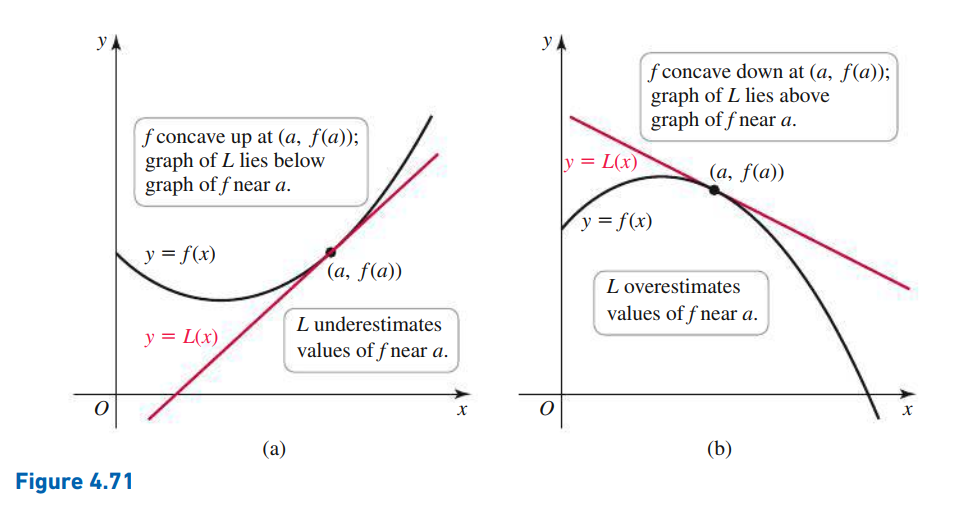
\includegraphics[scale=0.5]{images/briggs_04_06/fig4_71}
\end{center}

\begin{ex*}
  Find the linearization of the following functions at the given point and use concavity to identify if the linearization is an overestimate or an underestimate.
\end{ex*}
\begin{enumerate}[label=\alph*),itemsep=\stretch{1}]
  \item $f(x)=\dfrac{2}{x};\, a=1$
  \item $f(x)=e\inv[x];\, a=\ln(2)$
\end{enumerate}
\vspace*{\stretch{1}}
\pagebreak

%\noindent
%\fbox{\parbox{0.9875\linewidth}{
%  \textbf{Summary: Uses of Linear Approximation}
%  \begin{enumerate}
%    \item 
%      To approximate $f$ near $x=a$, use
%        $$f(x)\approx L(x)=f(a)+f'(a)(x-a).$$
%    \item 
%      To approximate the change $\Delta y$ in the dependent variable when the independent variable $x$ changes from $a$ to $a+\Delta x$, use
%        $$\Delta y\approx f'(a)\Delta x.$$
%  \end{enumerate}
%}}
%\pagebreak

%\begin{defn*}[Differentials]
%  
%  Let $f$ be differentiable on an interval containing $x$. A small change in $x$ is denoted by the \textbf{differential} $dx$. The corresponding change in $f$ is approximated by the \textbf{differential} $dy=f'(x)\,dx$. So if $\Delta x=dx$, where $\Delta x$ and $dx$ are both small, then $\Delta y\approx dy$:
%    \[\Delta y= f(x+dx)-f(x)\approx dy=f'(x)\,dx.\]
%    
%\end{defn*}

\begin{defn*}[Differentials]
    Let $f$ be a differentiable function on an interval containing $x$. An infinitesimal change in $x$ can be denoted by the \textbf{differential} $dx$. The corresponding change in the output of $f$ can be denoted by the \textbf{differential} $dy$. This yields the relation
        $$dy = f'(x)dx.$$
    Note that $dy$ and $dx$ can be thought of as the `rise' and `run' (respectively) of the line tangent to $f$ at the point $(x,f(x))$.
\end{defn*}

\begin{defn*}[$\Delta x$ and $\Delta y$]
    Let $f$ be a differentiable function on an interval containing $x$. We let $\Delta x$ denote a small change in $x$ and we let $\Delta y$ denote the corresponding change in $f(x)$. This yields the relation
        $$\Delta y = f(x+\Delta x) - f(x).$$
    Note that $\Delta y$ and $\Delta x$ can be thought of as the `rise' and `run' (respectively) of the secant line passing through the points $(x,f(x))$ and $(x+\Delta x, f(x+\Delta x))$.
\end{defn*}

\vspace*{\stretch{1}}
\noindent
\fbox{\parbox{0.9875\linewidth}{
  \textbf{Linear Approximation and Differentials}
    To approximate the change $\Delta y$ in the dependent variable when the independent variable $x$ changes from $x$ to $x+\Delta x$, use
        $$\Delta y\approx f'(x)\Delta x$$
    because if we set $\Delta x = dx$, then we have the following:
        $$\Delta y= f(x+\Delta x)-f(x)\approx f'(x)\,dx=dy.$$
    One can think of $\Delta y$ as the \textit{actual change} in the output of a function when $x$ changes by $\Delta x$, whereas $f'(x)\Delta x$ is the \textit{projected change} in the output of the function when the same $\Delta x$ is imposed. The point is these are approximately equal when $\Delta x$ is small.
}}
\vspace*{\stretch{1}}
\pagebreak

\begin{ex*}
  Find the differential $dy$.
\end{ex*}
\begin{tasks}[after-item-skip=\stretch{1}, label=~](2)
  \task $y=\cos(x^2)$
  \task $y=\sqrt{1-x^2}$
  \task $y=4x^2-3x+2$
  \task $y=x\tan(x^3)$
  \task $y=\cos^5(x)$
  \task $f(x)=\sin\inv(x)$
\end{tasks}
\vspace*{\stretch{1}}
\pagebreak
\begin{ex*}
  Let $y=x^2$
\end{ex*}
\begin{enumerate}[label=\alph*), itemsep=\stretch{1}]
  \item Find $dy$
  \item If $x=1$ and $dx=0.01$, find $dy$.
  \item Compare $dy$ and $\Delta y$ at this point.
\end{enumerate}
\vspace*{\stretch{1}}

\begin{ex*}
  Let $y=\sqrt{3+x^2}$
\end{ex*}
\begin{enumerate}[label=\alph*), itemsep=\stretch{1}]
  \item Find $dy$
  \item If $x=1$ and $dx=-0.1$, find $dy$.
  \item Compare $dy$ and $\Delta y$ at this point.
\end{enumerate}
\vspace*{\stretch{1}}

\pagebreak
\begin{ex*}
  Suppose $f$ is differentiable on $(-\infty,\infty)$ and $f(5.01)-f(5)=0.25$. Use linear approximation to estimate the value of $f'(5)$.
\end{ex*}
\vspace*{\stretch{1}}

\begin{ex*}
  Suppose $f$ is differentiable on $(-\infty,\infty)$ and $f(5.99)=7$ and $f(6)=7.002$. Use linear approximation to estimate the value of $f'(6)$.
\end{ex*}
\vspace*{\stretch{1}}
\pagebreak

\begin{ex*}
  Compute $dy$ and $\Delta y$ for $y=e^x$ when $x=0$ and $\Delta x=0.5$.
\end{ex*}
\vspace*{\stretch{1}}

\begin{ex*}
  Approximate the change in the area of a circle when its radius increases from $2.00$ to $2.02\,m$.
\end{ex*}
\vspace*{\stretch{1}}

\begin{ex*}
  Approximate the change in the magnitude of the electrostatic force between two charges when the distance between them increases from $r=20\,m$ to $r=21\,m$ $(F(r)=0.01/r^2$).
\end{ex*}
\vspace*{\stretch{1}}
\pagebreak

\begin{ex*}
  Approximate the change in the volume of a right circular cylinder of fixed radius $r=20\,cm$ when its height decreases from $h=12\,cm$ to $h=11.9\,cm$ ($V(h)=\pi r^2h$).
\end{ex*}
\vspace*{\stretch{1}}

\begin{ex*}
  Approximate the change in the volume of a right circular cylinder of fixed height $h=4\,m$ when its radius increases from $r=3\,m$ to $r=3.05\,m$ ($V(r)=\frac{1}{3}\pi r^2 h$).
\end{ex*}
\vspace*{\stretch{1}}
\pagebreak

\begin{ex*}
  The radius of a sphere is measured and found to be $0.7$ inches with a possible error in measurement of at most 0.01 inches.
\end{ex*}
\begin{enumerate}[label=\alph*), itemsep=\stretch{1}]
  \item What is the maximum error in using the value of the radius to compute the volume of the sphere?
  \item Find the relative error of the volume: \hfill\textit{relative error} $\dfrac{dV}{V}$\hspace*{50pt}
  
  What is the percentage error?
\end{enumerate}
\vspace*{\stretch{1}}
\pagebreak

\begin{ex*}
  The radius of a circular disk is given as $24\,cm$ with a maximum error in measurement of $0.2\,cm$.
\end{ex*}
\begin{enumerate}[label=\alph*), itemsep=\stretch{1}]
  \item Use differentials to estimate the maximum error in the calculated area of the disk.
  \item What is the relative error? What is the percentage error?
\end{enumerate}
\vspace*{\stretch{1}}
\pagebreak

\begin{ex*}
  Use differentials to estimate the amount of paint needed to apply a coat of paint $0.05\,cm$ thick to a hemispherical dome with diameter $50\,m$.
\end{ex*}
\vspace*{\stretch{1}}
\pagebreak
\end{document}
